
\subsubsection{5.1 Attention Concentration in Llama-2-7B (RQ2, Confirmed)}

Experiment h-e1 characterizes within-layer attention concentration across 200 evaluation examples drawn from the LongBench hotpotQA subset. Attention weight concentration is measured using the Gini coefficient and top-10\% token share, computed via head-mean pooling across all 32 attention heads.

\textbf{Table 1: Attention Concentration Statistics (h-e1, N = 200 evaluation examples)}

\begin{table*}[htbp]
\centering
\resizebox{\dimexpr 2\columnwidth+\columnsep\relax}{!}{%
\begin{tabular}{lllll}
\toprule
Metric & Mean & Std & Gate Threshold & Satisfaction Rate \\
\midrule
Gini Coefficient & 0.6829 & 0.0117 & > 0.5 & 100\% (200/200) \\
Top-10\% Token Share & 0.7172 & 0.0196 & > 0.5 & 100\% (200/200) \\
Both criteria simultaneously & --- & --- & Both satisfied & 100\% (200/200) \\
\bottomrule
\end{tabular}
}
\end{table*}

The Gini coefficient of 0.6829 indicates that attention weight is highly concentrated in a minority of tokens. Both criteria are satisfied by all 200 evaluation examples without exception. The low standard deviations (0.0117 and 0.0196) indicate that this concentration pattern is consistent across diverse examples within this evaluation domain.

These findings confirm that Llama-2-7B does not perform uniform global attention --- attention weight is highly unequal in distribution, with the top 10\% of tokens capturing an average of 71.72\% of the total weight. This heavy-hitter pattern is the empirical basis for the hypothesis that high-entropy layers --- those with more diffuse distributions --- may tolerate SWA constraints.

\begin{figure}[htbp]
\centering
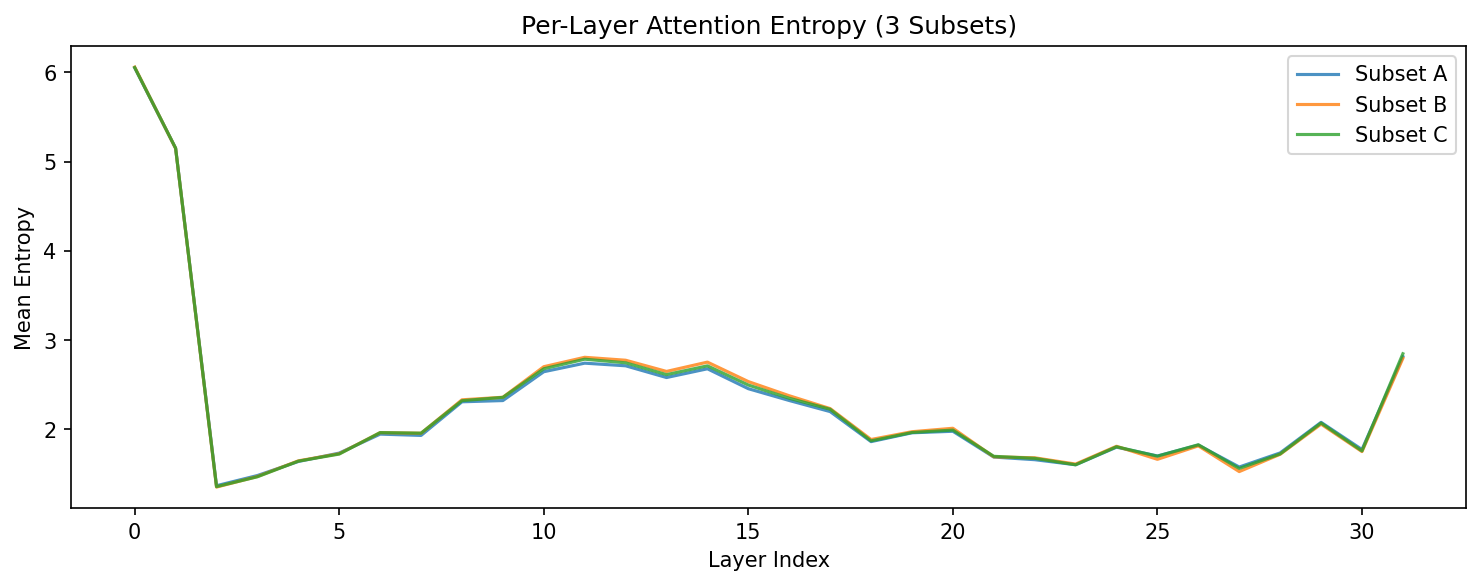
\includegraphics[width=\columnwidth]{figures/layer_entropy_per_subset.png}
\caption{Layer entropy per calibration subset}
\label{fig:layer_entropy_per_subset}
\end{figure}

\textit{Figure 1: Per-layer entropy profiles across calibration subsets, illustrating consistency of the entropy curve shape across the 32 layers of Llama-2-7B.}

\begin{figure}[htbp]
\centering
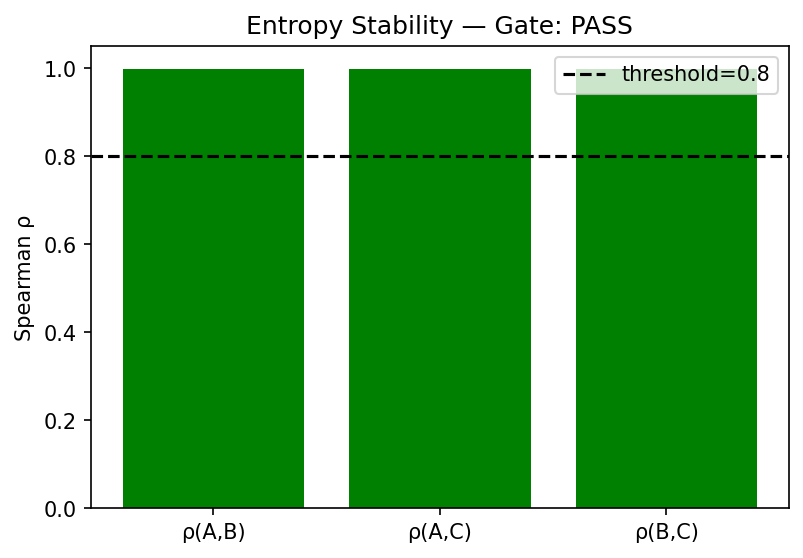
\includegraphics[width=\columnwidth]{figures/entropy_stability.png}
\caption{Entropy stability across examples}
\label{fig:entropy_stability}
\end{figure}

\textit{Figure 2: Attention concentration (Gini coefficient and top-10\% token share) across 200 evaluation examples, illustrating within-domain consistency.}

\subsubsection{5.2 Entropy Ranking Stability (RQ1, Confirmed)}

\textbf{Table 2: Spearman Rank Correlation Across Calibration Subsets (h-e1)}

\begin{table}[htbp]
\centering
\resizebox{\columnwidth}{!}{%
\begin{tabular}{lll}
\toprule
Subset Pair & Spearman $\rho$ & Gate Criterion \\
\midrule
A vs. B & $\geq$ 0.8 & $\rho \geq$ 0.8 ✓ \\
A vs. C & $\geq$ 0.8 & $\rho \geq$ 0.8 ✓ \\
B vs. C & $\geq$ 0.8 & $\rho \geq$ 0.8 ✓ \\
min($\rho_{AB}$, $\rho_{AC}$, $\rho_{BC}$) & $\geq$ 0.8 & GATE: PASS ✓ \\
\bottomrule
\end{tabular}
}
\end{table}

\textit{Note: Exact per-pair $\rho$ point estimates were confirmed to satisfy the $\geq$ 0.8 gate criterion, but are not separately tabulated in the available h-e1 output files. The gate verdict (PASS) is confirmed. Per-pair values should be extracted from h-e1 implementation logs before final submission.}

The entropy criterion produces stable layer rankings across independent calibration subsets, confirming that the selected top-k layers are not sensitive to which specific 100 sequences are used for calibration.

\begin{figure}[htbp]
\centering
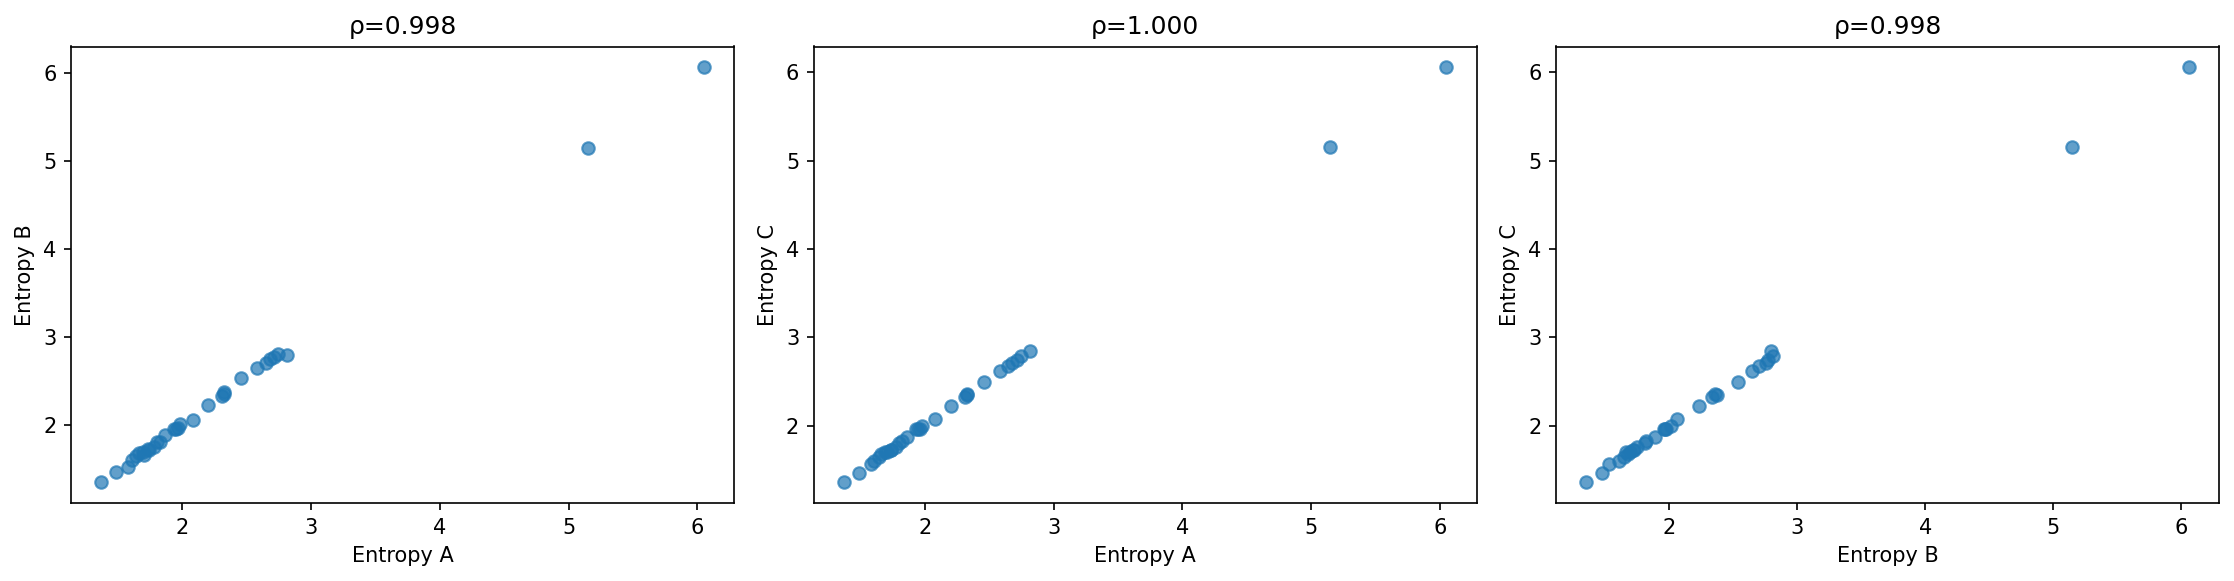
\includegraphics[width=\columnwidth]{figures/rank_correlation_scatter.png}
\caption{Rank correlation scatter}
\label{fig:rank_correlation_scatter}
\end{figure}

\textit{Figure 3: Pairwise scatter plots of per-layer entropy scores across calibration subsets, illustrating ranking stability (Spearman $\rho \geq$ 0.8 for all pairs).}

\begin{figure}[htbp]
\centering
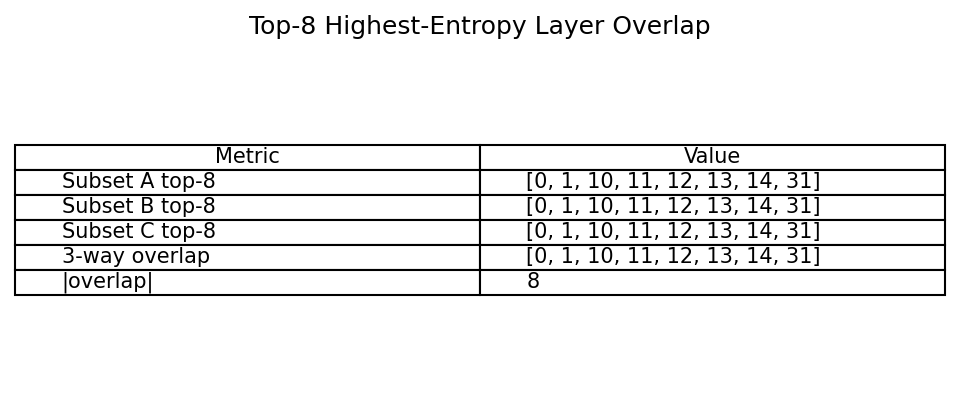
\includegraphics[width=\columnwidth]{figures/top8_overlap.png}
\caption{Top-8 layer overlap}
\label{fig:top8_overlap}
\end{figure}

\textit{Figure 4: Overlap in top-8 highest-entropy layers across calibration subsets, visualizing selection determinism.}

\subsubsection{5.3 Head-Mean vs. Head-Max Pooling (RQ3, Confirmed)}

\textbf{Table 3: Pooling Method Comparison for Layer-Level Entropy Concentration (h-e1)}

\begin{table}[htbp]
\centering
\resizebox{\columnwidth}{!}{%
\begin{tabular}{lll}
\toprule
Pooling Method & Mean Gini & Interpretation \\
\midrule
Head-mean (used in this work) & 0.681 & Captures layer-level structural property across all heads \\
Head-max & 0.466 & Dominated by single outlier heads per layer \\
Relative difference & $-32$\% (head-max vs. head-mean, denominator = head-mean) & Head-mean produces substantially higher measured concentration \\
\bottomrule
\end{tabular}
}
\end{table}

\textit{Note: The $-32$\% figure is (0.681 - 0.466) / 0.681 = 31.6\% $\approx$ 32\%, using head-mean as the denominator. Equivalently, head-mean Gini is 46.1\% higher than head-max Gini when head-max is the denominator: (0.681 $-$ 0.466) / 0.466 = 46.1\%. The head-max ablation was computed over 10 examples.}

Head-mean pooling captures a substantially larger concentration signal than head-max. This gap arises because head-max reports the single highest-entropy head in each layer --- a noisy outlier measure --- rather than the average behavior shared across all 32 heads. For any entropy-based layer characterization method, this methodological choice has measurable impact on signal quality.

\subsubsection{5.4 Exploratory Attention Span Probe (Non-Significant, for Transparency)}

As an exploratory addition to h-e1, a preliminary probe compared entropy-guided attention span selection against random selection on a QA F1 task using attention truncation (top-k retained scores, not SWA masking). Entropy selection degraded QA F1 by 0.43 percentage points, versus 0.67 pp for random selection ($\Delta$ = 0.24 pp advantage for entropy). This difference was not statistically significant (p = 0.4507, paired t-test, N = 200). The operation (top-k score retention) and metric (QA F1) differ from the designed h-m1 experiment (SWA masking, WikiText-103 perplexity). This result is reported for transparency only and does not constitute evidence for entropy-guided selection superiority over random selection.

\textbf{Table 4: QA F1 Under Attention Truncation (h-e1 Exploratory Probe)}

\begin{table}[htbp]
\centering
\resizebox{\columnwidth}{!}{%
\begin{tabular}{lll}
\toprule
Condition & Mean F1 & Delta vs. Full Cache \\
\midrule
Full cache & 0.0274 & --- \\
Entropy top-20 & 0.0273 & $-0.0001$ pp \\
Entropy top-40 & 0.0231 & $-0.43$ pp \\
Random top-20 & 0.0239 & $-0.34$ pp \\
Random top-40 & 0.0206 & $-0.67$ pp \\
P2 comparison (attn40 vs. rand40) & 0.43 pp vs. 0.67 pp & p = 0.4507 (non-significant) \\
\bottomrule
\end{tabular}
}
\end{table}

\subsubsection{5.5 Entropy-Guided SWA Conversion: WikiText-103 Perplexity (RQ4, Confirmed)}

Experiment h-e2 applies entropy-guided k = 4 SWA conversion to Llama-2-7B and evaluates WikiText-103 test perplexity.

\textbf{Entropy scores.} The calibration pass (n = 100 sequences, processing terminated after 63 sequences) produced entropy scores across all 32 layers. The two highest-entropy layers were layers 0 and 1, with scores of 3.201 and 2.972 --- substantially higher than all other layers. The third and fourth highest were layer 31 (score 1.770) and layer 10 (score 1.687). The remaining 28 layers had entropy scores between approximately 0.90 and 1.63.

\textbf{Selected layers:} [0, 1, 10, 31]. Depth distribution: 2 early (layers 0--1), 1 mid (layer 10), 1 late (layer 31).

\textbf{Table 5: WikiText-103 Perplexity Results (h-e2)}

\begin{table}[htbp]
\centering
\resizebox{\columnwidth}{!}{%
\begin{tabular}{llll}
\toprule
Condition & PPL & $\Delta$ PPL vs. Baseline & Gate ($\Delta \leq$ 2.0) \\
\midrule
Full attention (baseline) & 6.3386 & --- & --- \\
Entropy-guided k = 4 SWA(w = 512) & 6.3226 & $-0.016$ & PASS ✓ \\
\bottomrule
\end{tabular}
}
\end{table}

The entropy-guided k = 4 SWA conversion results in a perplexity of 6.3226, versus a full-attention baseline of 6.3386. The difference is $-0.016$ points (a negligible improvement rather than degradation), satisfying the $\leq$ 2.0-point gate criterion with a substantial margin. This confirms that selectively converting the 4 highest-entropy layers to SWA(w = 512) does not meaningfully alter language modeling quality on WikiText-103, under the zero-shot condition (no fine-tuning).

\textbf{Implementation note.} Mask validation confirmed correct SWA mask construction. The mechanism verification check (comparing attended positions against the expected window size) produced an informational warning in the first run because the hook measured the pre-patch mask state; the second run confirmed mechanism activation via non-zero PPL delta (|$\Delta |$ = 0.016 $\neq$ 0), indicating that the SWA patches were active during evaluation. The swa\_patch implementation replaces \texttt{attention\textbackslash \_mask} with the SWA mask for each selected layer's forward call.

\begin{figure}[htbp]
\centering
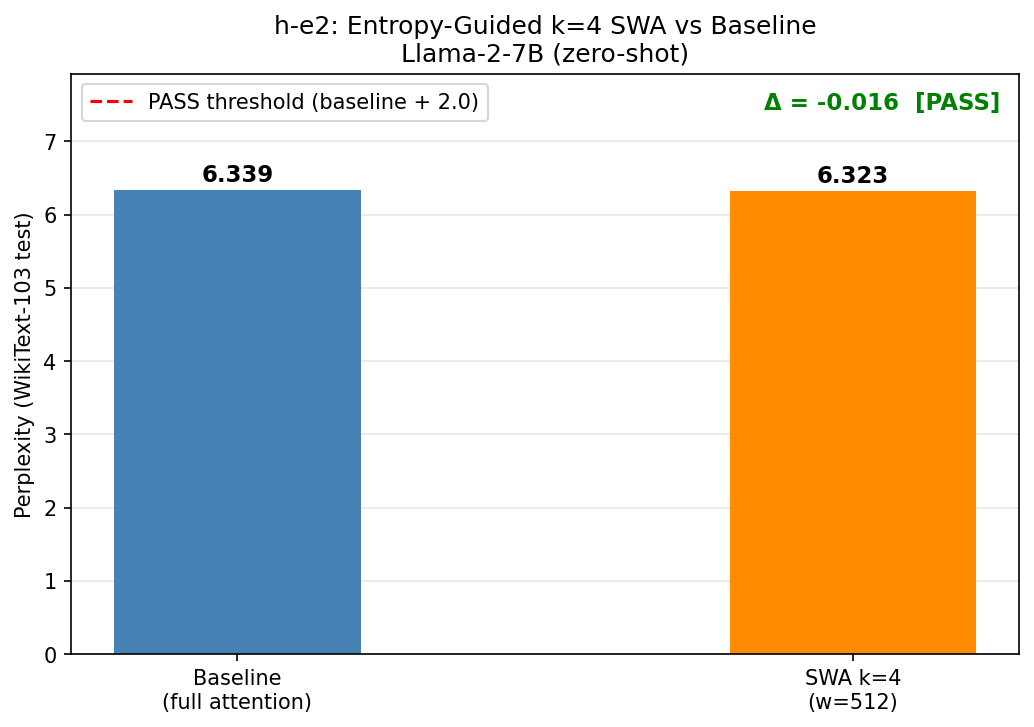
\includegraphics[width=\columnwidth]{figures/ppl_comparison.png}
\caption{Perplexity comparison}
\label{fig:ppl_comparison}
\end{figure}

\textit{Figure 5: WikiText-103 perplexity comparison between the full-attention baseline and entropy-guided k = 4 SWA conversion. The 2.0-point threshold (gate criterion) is shown as a reference line. The observed $\Delta = -0.016$ is well within the threshold.}

\begin{figure}[htbp]
\centering
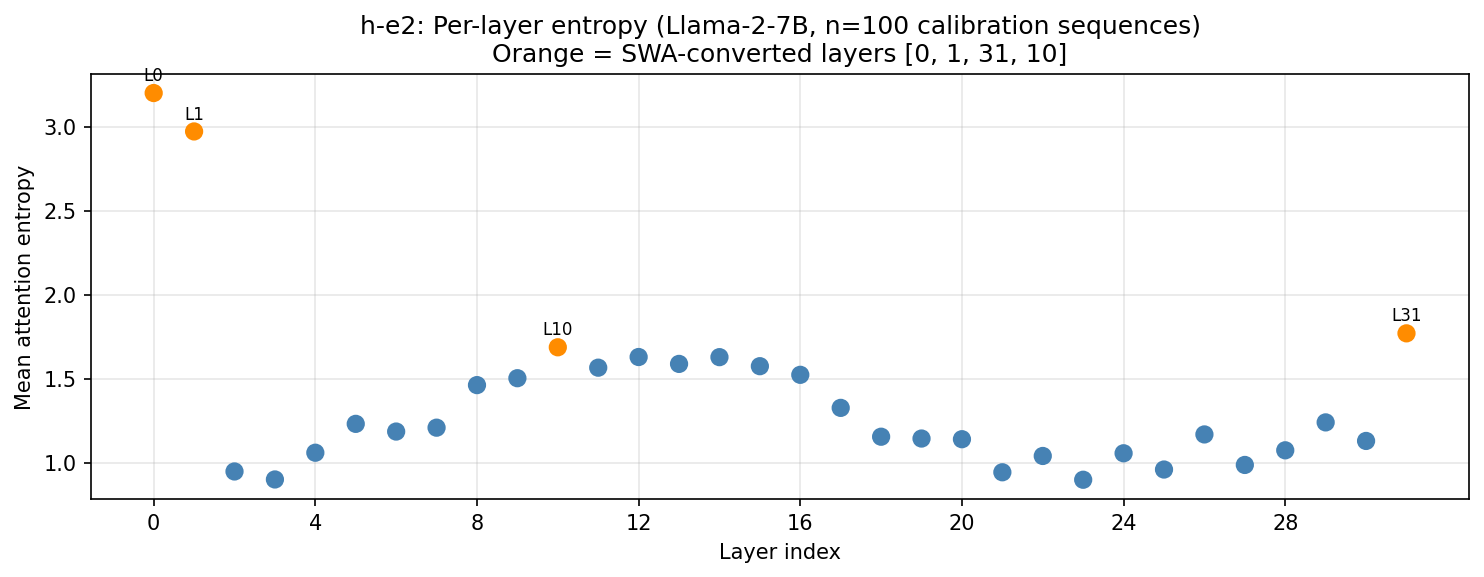
\includegraphics[width=\columnwidth]{figures/entropy_scatter.png}
\caption{Entropy scatter across layers}
\label{fig:entropy_scatter}
\end{figure}

\textit{Figure 6: Per-layer entropy scores from the h-e2 calibration pass. Layers 0 and 1 exhibit markedly higher entropy (3.20 and 2.97) relative to all other layers (range 0.90--1.77). Selected layers are indicated.}

\subsubsection{5.6 Planned Experiments (Not Yet Executed)}

The following comparisons are designed and ready to execute but have not been run:

\textbf{Table 6: Planned Comparisons (Execution Pending)}

\begin{table}[htbp]
\centering
\resizebox{\columnwidth}{!}{%
\begin{tabular}{llll}
\toprule
Experiment & Condition & Metric & Status \\
\midrule
h-m1 & Random-k = 4 SWA (mean 3 seeds) & $\Delta$ PPL vs. baseline & Not executed \\
h-m1 & Last-k = 4 SWA (layers 28--31) & $\Delta$ PPL vs. baseline & Not executed \\
h-m1 & Entropy vs. random superiority & p-value (Wilcoxon) & Not executed \\
h-m2 & Entropy-guided k = 8 SWA & $\Delta$ PPL vs. k = 4 & Not executed \\
\bottomrule
\end{tabular}
}
\end{table}

No superiority claims over random or last-k selection are made without executed comparison data.

